%% The following is a directive for TeXShop to indicate the main file
%%!TEX root =../diss.tex

\chapter{Interlude}
\label{ch:interlude}
Through the course of the preceding work, it quickly became evident that not only is tumour oxygenation a key feature of the microenvironment, but that there is also a dearth of non-invasive techniques available to measure it.
Below we introduce some background information around the use of oxygen as a contrast agent, as well as some physiological information that may be relevant to develop a new MR-based method to assess oxygenation.
To explore the mechanism of action for the oxygen-enhanced MRI signal, it is useful to first understand the delivery of oxygen from inspired air to tissues.

 \section{Theory}
 To explore the mechanism of action for the OE-MRI signal, it is useful to first understand the delivery of oxygen from inspired air to tissues. 
 The primary mode of oxygen delivery to tissue is the haemoglobin (\acs{Hb}) molecule as it carries and delivers 98\% of the oxygen in the body. 
 Over 250 million \acs{Hb} molecules are found in a typical red blood cell and each \acs{Hb} molecule has four binding sites for oxygen molecules. 
 The binding affinity of \acs{Hb} to bind ${O_2}$ increases 

 The binding affinity for ${O_2}$ drastically increases for subsequent oxygen molecules that bind to \acs{Hb} as the conformation of the \acs{Hb} molecule changes to increase binding affinity for the next oxygen, a phenomenon called cooperativity. 
 Similarly, when the partial pressure of ${O_2}$ is lower, bound ${O_2}$ is released 

 when the local environment of the \acs{Hb} molecule changes such that ${O_2}$ needs to be released, the reverse conformational changes occur so a proportionately lower drop in oxygen tension is required to release the next ${O_2}$ molecule. 

 \section{Physiology}

 The primary mode of oxygen delivery to tissue is the haemoglobin (\acs{Hb}) molecule as it carries and delivers 98\% of the oxygen in the body. 
 Over 250 million \acs{Hb} molecules are found in a typical red blood cell and each \acs{Hb} molecule has four binding sites for oxygen molecules. 
 The binding affinity for ${O_2}$ drastically increases for subsequent oxygen molecules that bind to \acs{Hb} as the conformation of the \acs{Hb} molecule changes to increase binding affinity for the next oxygen, a phenomenon called cooperativity. 
 Similarly, when the local environment of the \acs{Hb} molecule changes such that O$_2$ needs to be released, the reverse conformational changes occur; a proportionately lower drop in oxygen tension is then required to release the next O$_2$ molecule. 
 The dissociation of oxygen from haemoglobin molecules is well described by the oxygen-haemglobin dissociation curve (figure~\ref{HBdis}).

% 	\begin{figure}
% 		\begin{center}
% 		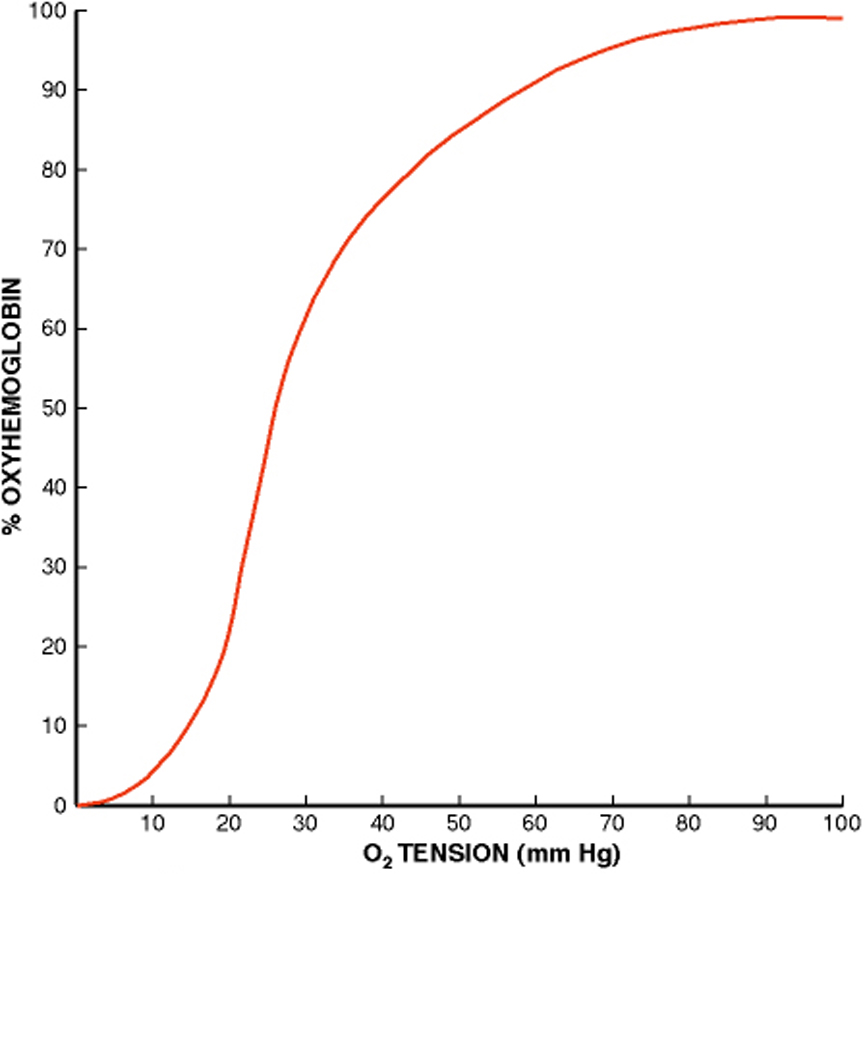
\includegraphics[width=\textwidth]{./intro/intro-images/HBdis.png}
% 		\caption{Sigmoidal curve illustrating the relationship between the haemoglobin saturation (y-axis) and the oxygen tension (x-axis). Note that the curve is very steep in the middle but it takes a large increase in oxygen tension to bind the last O$_2$ and similarly, a large decrease in oxygen tension to release the last  O$_2$~\cite{GomezCambronero:2001hu}.}
% 		\label{HBdis}
% 		\end{center}
% 	\end{figure}	

 Upon inspiration of atmospheric air (p$_{O_2}$ = 160 mmHg), gas exchange in the pulmonary capillary beds occurs in the alveoli of the lungs (Fig~\ref{mmhg}).
 Incoming venous blood with a low oxygen tension (p$_{O_2}$ = 40 mmHg) is oxygenated as haemoglobin molecules readily bind available oxygen. 
 As the oxygenated blood leaves the alveoli and moves through the systemic arteries, it has an oxygen tension of 100 mmHg. 
 The oxygenated blood then travels from the arteries to the systemic capillary bed and the local oxygen tension drops from 100 to 40 mmHg.
 Simultaneously, while the \acs{Hb} molecule undergoes a structural change releasing a molecule of O$_2$ from its first binding site.  
 The second release of the oxygen molecule occurs when the tension drops to 26mmHg~\cite{GomezCambronero:2001hu}. 
 The third and fourth molecules are released with consecutively smaller drops in oxygen tension as low oxygen tension indicates an oxygen starved environment. This important feature of \acs{Hb} (cooperativity) ensures that small changes in p$_{O_2}$ have the appropriate effect in the appropriate place. 
 For instance, in the lung tight binding is required so \acs{Hb} can bind the O$_2$ needed to supply all the tissues.
 Therefore, small changes should not affect the release of O$_2$.
 Conversely, small changes in p$_{O_2}$ in capillary beds should result in quick release of O$_2$ so it can easily diffuse to oxygen-starved tissues. 
 Practically however, it is important to note that \acs{Hb} molecules never release all four of the bound oxygen.

% 	\begin{figure}
% 		%\begin{center}
% 		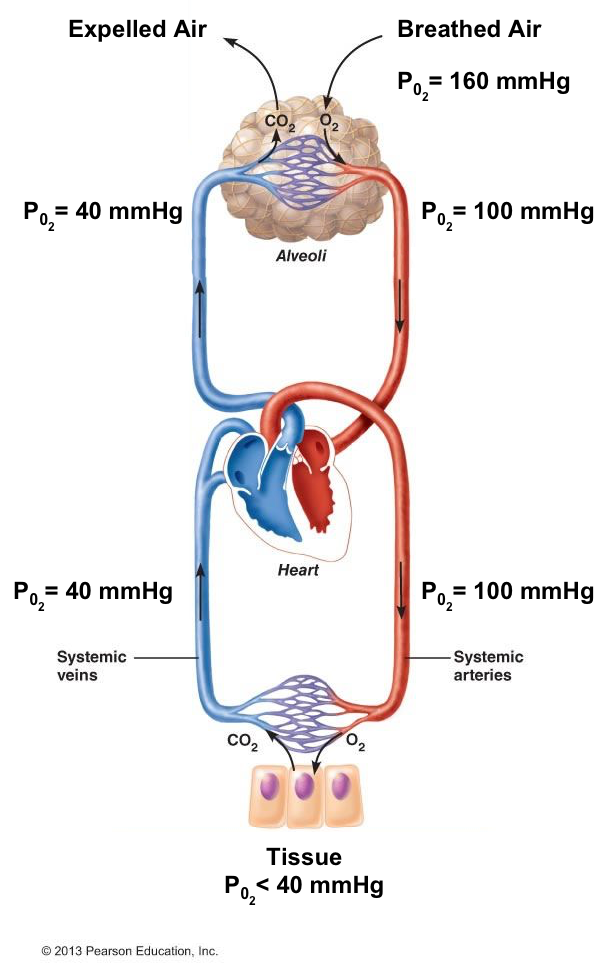
\includegraphics[width=0.8\textwidth]{./intro/intro-images/mmHg.png}
% 		\caption{A schematic of the oxygen/\acs{Hb} transport mechanism through the system blood stream. Photo credit: Pearson Education, Inc. 2013}
% 		\label{mmhg}
% 		%\end{center}
% 	\end{figure}

 \section{Origin of the OE-MRI Signal}

 Oxygen is a paramagnetic molecule because it has two unpaired electrons and it is widely reported that the dominating effect in the OE-MRI signal is a T$_1$ decrease after concentrated oxygen gas (100\% O$_2$) is breathed in~\cite{OConnor:2016ee,Linnik:2013hf}. 
 The excess oxygen travels through the blood stream dissolved in plasma and diffuses through the vessel walls and dissolves in interstitial tissue fluid (figure~\ref{oemri}).
 The net increase in dissolved oxygen results in a dramatic and measurable decrease in T$_1$. 
 This change is reversed soon after the patient is switched back to breathing atmospheric air as excess oxygen is expelled or metabolized. 
 Perfused tumour regions (i.e regions that already have a high \acs{Hb}-O$_2$ saturation) will see a measurable decrease in T$_1$. 
 The perfused regions that do not show a decrease in T$_1$ must therefore be hypoxic~\cite{OConnor:2016ee}. 
 Importantly, OE-MRI does not yield any information about unperfused regions and in that region, there are likely to be pockets of viable (but hypoxic) tissue.

 The oxygen status of healthy tissue is fairly well regulated in normal tissue and every cell in the body is at most 150$\mu$m away from a blood vessel. 
 In tumours however, the vascular network is chaotic and the growth patterns of vessels are abnormal leading to a defective and leaky endothelium~\cite{McDonald:2002ut}. 
 Irregular diameters of tumour vessels, abnormal branching patterns and leaky vessel walls all contribute to an increase in vessel permeability and pockets of hypoxic tissue. 
 Unfortunately in hypoxic tissue the oxygen status cannot be well characterized as many factors can influence the oxygen dissociation curve including temperature, pH, and carbon dioxide concentration - all factors that persist unregulated in tumour hypoxic tissue. 
 Furthermore, these hypoxic regions are heterogeneous, transient, and drastically differ between tumour models. 
 Thanks to some excellent work with spectral imaging using an implanted window chamber in mice, it is known that upon breathing 100\% oxygen, the \acs{Hb} saturation in the tumour vascular network increases from 20-30\% up to 70-80\% while the \acs{Hb} saturation in the normal vascular network does not change appreciably~\cite{Sorg:2008eg}.
 \SARi{I would present this as a tentative model that we have. You can update the picture to show some of our most recent refinments in the understanding ...}

 \todo{Should probably discuss whether this (admittedly flawed) picture of our understanding should still be included, or the waterton figure re-created}
%    	\begin{figure}
%    		\begin{center}
%    		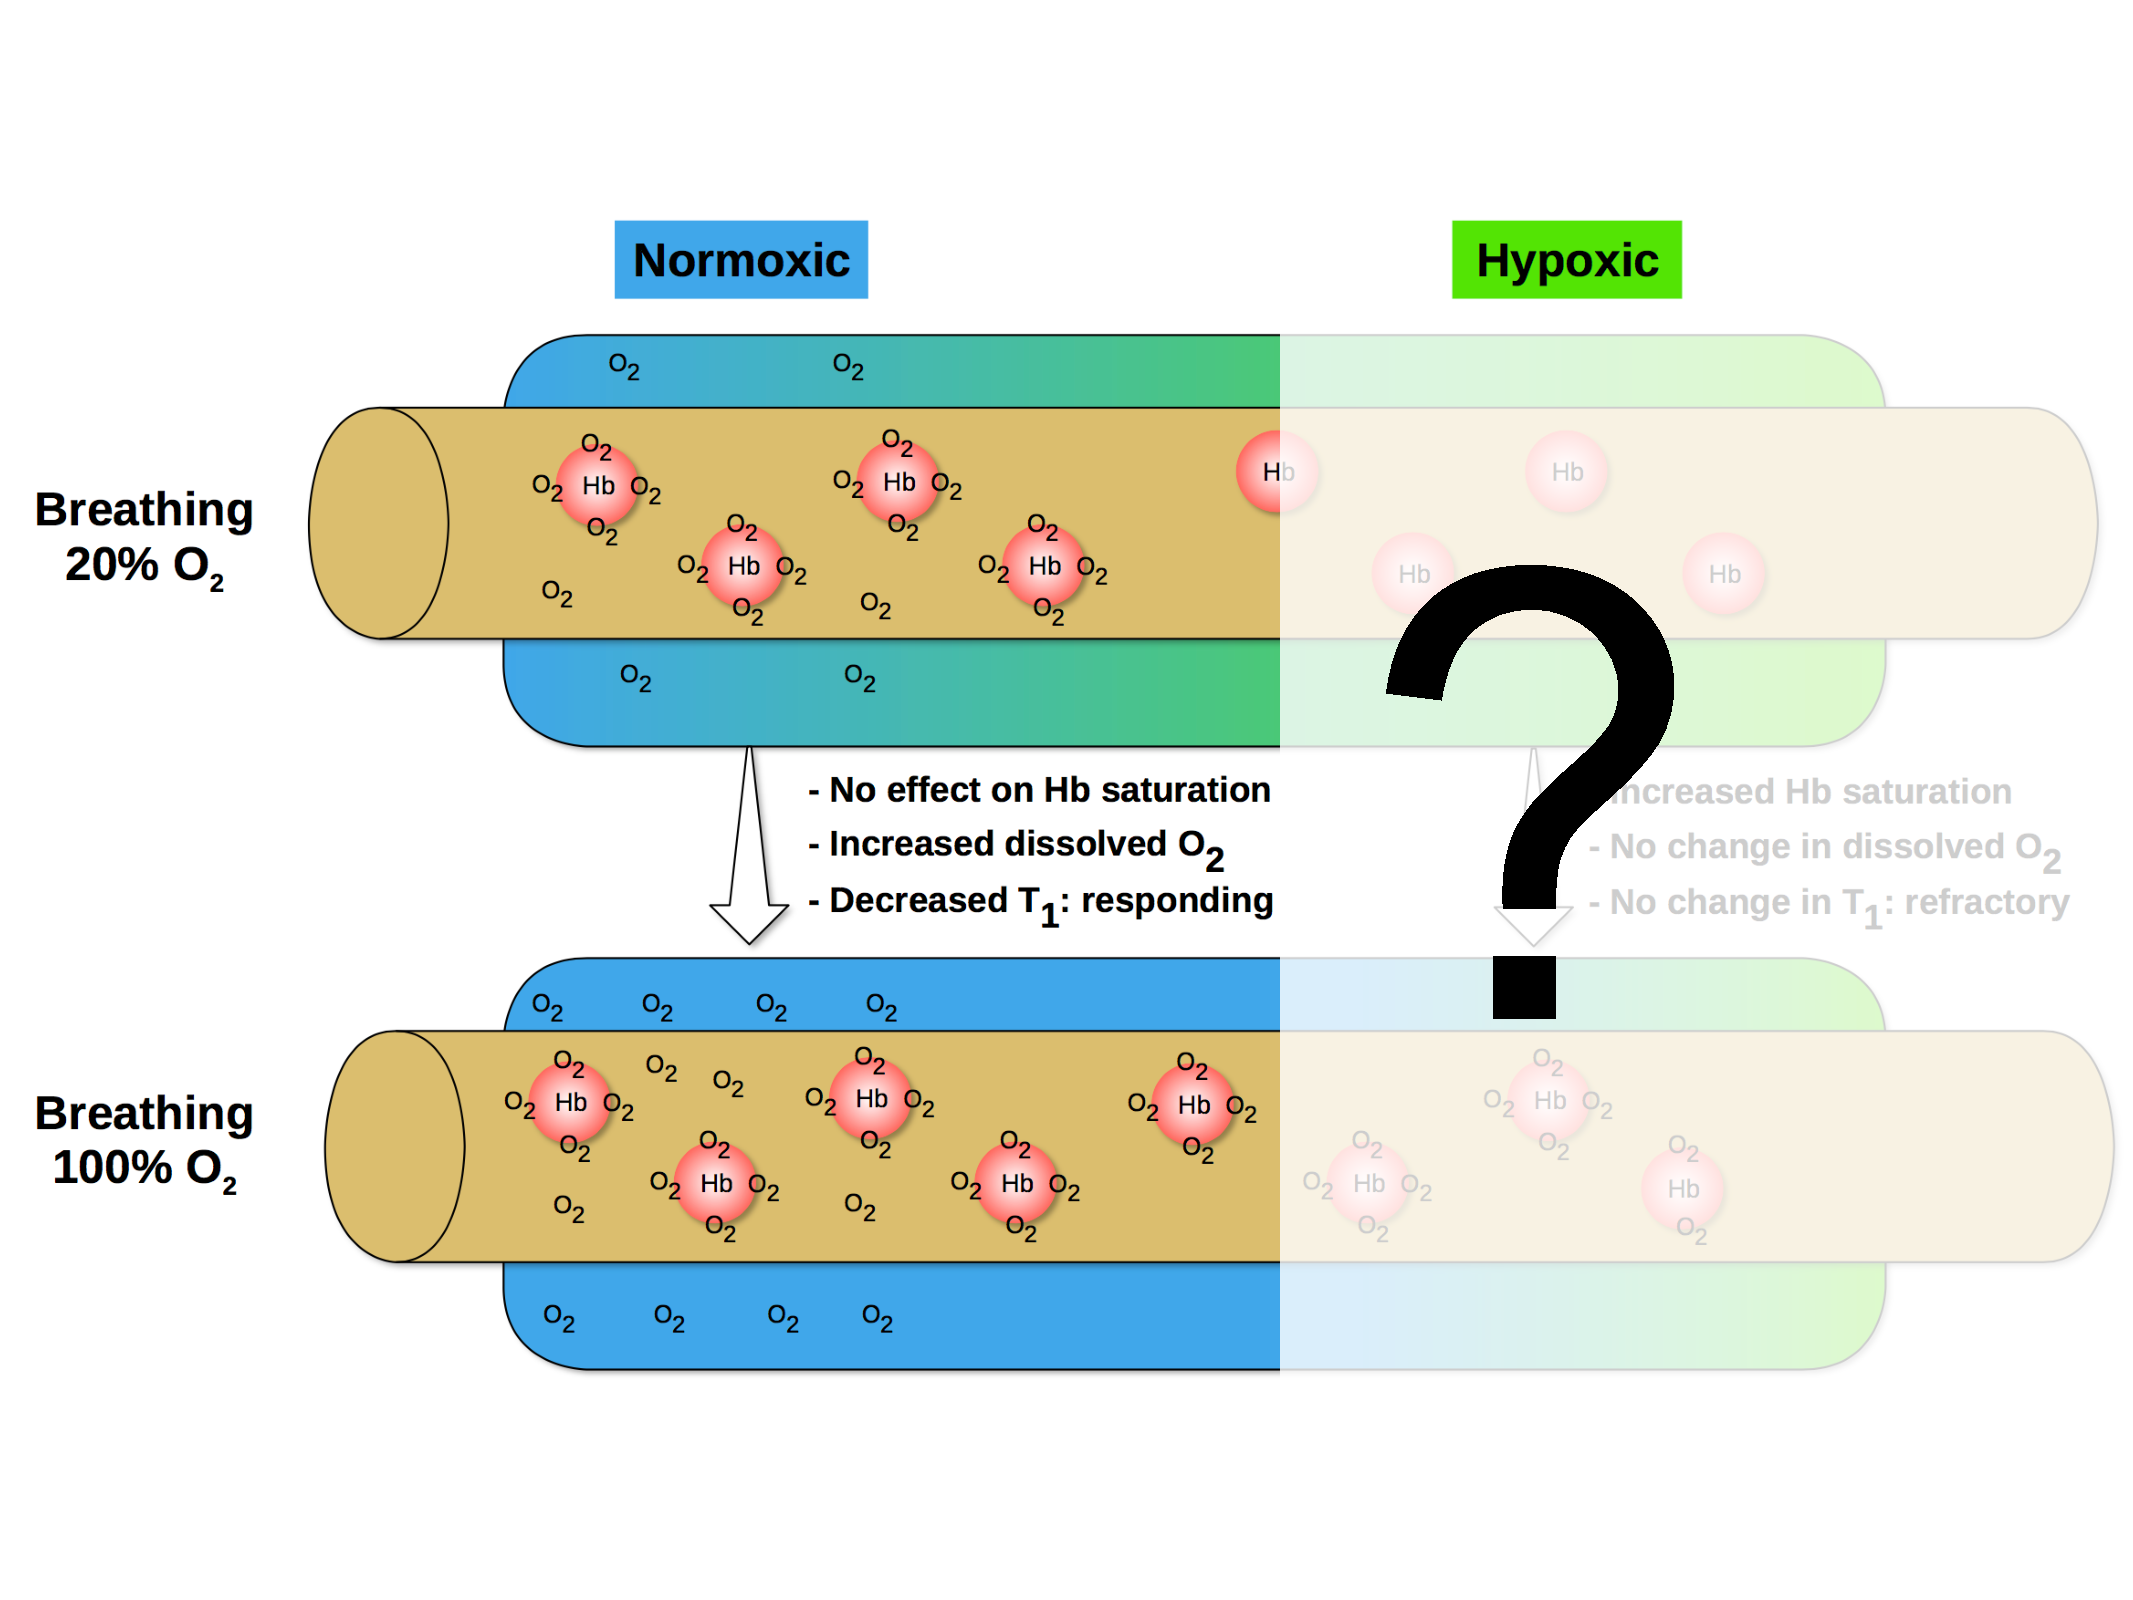
\includegraphics[width=\textwidth]{./intro/intro-images/oemriDark.pdf}
%    		\caption{A schematic representation of the origin of the OEMRI effect. In normoxic tissue, \acs{Hb} is almost fully saturated and any excess breathed O$_2$ cannot bind to the \acs{Hb} molecule. Consequently, O$_2$ dissolves in the blood plasma and as the excess oxygen diffuses out into the tissue, it also dissolves in the interstitial tissue fluid resulting in a net T$_1$ decrease. It is hypothesized that in the hypoxic tissue, \acs{Hb} is not fully saturated with oxygen due to increased tissue demands and/or a poorly organized vascular network. The excess breathed oxygen in this case binds to the \acs{Hb} molecule and does \textbf{not} dissolve in the plasma leading to no change in T$_1$.}
%    		\label{oemri}
%    		\end{center}
%    	\end{figure}

